\documentclass[a4paper, 10pt, conference]{IEEEtran}      % For A4 Paper
%The Class IEEECONF will be installed by MiKTeX and Texmaker automatically
% All the required Packages will be automatically installed if you have MiKTeX and Texmaker 
\usepackage{algorithm,algpseudocode}

\usepackage{amsmath}
\usepackage{amssymb} 
\usepackage{graphics}
\usepackage{epsfig}
\usepackage{mathptmx}
\usepackage{array}
\usepackage{tabu}
\usepackage{hyperref}
% If You use Texmaker it will automatically download missing packages

\title{\LARGE \bf OpenMP: Earthquake Simulation}
% Enter your Title here
% If the title is too long use line breaker (\\) to break into two
% If you do not use line breaker manually, it will be broken automatically by LATEX  

\author{Chirag Majithia}

\begin{document}
	
	
	\maketitle
	\thispagestyle{empty}
	\pagestyle{empty}
	
	
	
	\begin{abstract}
		The aim of the project is to get familiarized to OpenMP API used for multi-platform shared-memory parallel programming in C/C++/Fortran. Here we parallelize benchmarked quake simulation code by Loukas Kallivokas and David O'Hallaron.
		
	\end{abstract}
	
	
	
	\section{Earthquake Simulation}
	
	Given is the code used as a benchmark for simulating earthquake by Loukas Kallivokas and David O'Hallaron and later by Wes Jones, SGI for Standard Performance Evaluation Corporation. The task is to use OpenMP API to parallelize the code and evaluate it's performance with the original code.
	In order to understand which parts of the sequential code need speed-up by parallelizing, we use GNU profiling tool (GPROF). Then we use various OpenMP directives to debug and parallelize the code which are discussed in the section \ref{ompdir} and the evaluation of the performance is discussed in section \ref{eval}. 
	
	\section{Profiling the sequential program}
	
	Profiling is an important aspect of software programming. Through profiling one can determine the parts in program code that are time consuming and need to be re-written. This helps make your program execution faster which is always desired.
	
	We run GPROF on the sequential code provided to us and get following result (refer table \ref{profile}):
	
	\begin{table}[H]
		
		
		\caption{gprof output: Flat profile:}
		\label{profile}
		\begin{tabu} to \linewidth { | X[c] | X[c] |  X[c] | X[c] | X[c] |}
			\hline
			\hline
		  percentage & cumulative & self  &  &    \\           
		time  & seconds &  seconds &   calls   & name \\   
		\hline
		64.48  &   42.80  &  42.80 &    3855 &  smvp \\
		\hline
		31.74  &   63.86 &   21.07   &  & main\\
		\hline
		1.14   &  64.62  &   0.76 &348904485  & phi2\\
		\hline
		1.05   &  65.31  &   0.70 &348904485  &  phi0\\
		\hline
		0.78   &  65.83  &   0.52 &348904485  &  phi1\\
		\hline
		0.35   &  66.06  &   0.23 &  151173   &  elemt\_mat\\
		\hline
		\hline
		
		\end{tabu}
	\end{table}

	As indicated by the profiler, \ref{profile}, it is clear that the functions smvp and main took majority of computation time. Thus, on analyzing the section of code, various for loops in these two function were found to be easily parallelize.

	\section{OpenMP Directives} \label{ompdir}
	
	Following OpenMP directives were used:
	\subsection{parallel}
	When a thread reaches a \textit{parallel} directive, it creates a team of threads (Fork) and becomes the master of the team. The master is a member of that team and has thread number 0 within that team.
	Starting from the beginning of this parallel region, the code is duplicated and all threads will execute that code. There is an implied barrier at the end of a parallel region (Join). Only the master thread continues execution past this point. If any thread terminates within a parallel region, all threads in the team will terminate, and the work done up until that point is undefined.
	
	\subsection {for}
	The \textit{for} directive specifies that the iterations of the loop immediately following it must be executed in parallel by the team. This assumes a parallel region has already been initiated, otherwise it executes in serial on a single processor.
	
	\subsection{parallel for}
	OpenMP provides \textit{parallel for} directive as a convenience substitute to an individual \textit{parallel} directive being immediately followed by \textit{for} directive.
	
	\section {OpenMP Clause}
	
	\subsection{Data Scope Attribute Clauses}
	\subsubsection{Shared}
	The \textit{shared} clause declares variables in its list to be shared among all threads in the team. A shared variable exists in only one memory location and all threads can read or write to that address.\\
	
	\subsubsection{Private}
	The variables declared \textit{private} become a new object of the same type for each thread in the team (uninitialized). All references to the original object are replaced with references to the new object. The scope of these new variable is limited to the parallel region are lost as soon as the team  joins back to the master thread.\\
	
	\subsubsection{Default}
	
	The \textit{default} clause allows the user to specify a default scope for all variables defined before the parallel region and extends it to the parallel region. That is, if the default scope of a variable is \textit{shared}, all the pre-defined variable upto the start of parallel region, remain shared in the parallel region. (There is no support of \textit{default private} and \textit{default first private} in C/C++). The clause used during the project is default \textit{\textbf{None}}. This directive requires that the programmer explicitly scope all variables.
	 
	 A race condition is an undesirable situation that occurs when a device or system attempts to perform two or more operations  on a single variable at the same time. This race conditions are caused by shared variables that really should have been declared private. Start by looking at the variables inside the parallel regions and make sure that the variables are declared private when necessary. It was used to debug the parallel construct at line ~ 287 in the sequential code, which created erroneous results.
	 
	 By default, all the variables are \textit{shared}.\\
	 
	\subsubsection{First Private}
	The \textit{firstprivate} clause combines the behavior of the \textit{private} clause with automatic initialization of the variables in its list, with the value of their original objects prior to entry into the parallel or work-sharing construct.\\
	
	\textit{firstprivate} was used at various places in code - especially places where there was a pre-initialized variable modified in the parallel construct with some computation using its previous value. However, there were instances in the code, where using \textit{firstprivate} instead of \textit{shared} speed up the computation time, even though the variable in use was just used to assign values to other variables. \\
	
	\subsection{Section Clauses}
	\subsubsection{NoWait}
	A parallel construct starts a parallel block. This forks a team of thread with in the constructs and all of them join at the end of the construct. However, a parallel construct may have various sections/for loops. Thus at  beginning of each loop or section, the master thread  delegates portions of the loop for different threads in the current team. All the threads wait at the end of loop to begin the next section (implicit barrier). However, if the subsequent for loops within the construct are independent of the variables used in the previous, the programmer can direct the threads to not wait for other threads at the end of the loop and move forward with the next execution. This override of implicit barrier is done using \textbf{NoWait} clause.
	It was used in mem\_init and initialization phase of the main loop.\\
	
	\subsubsection{Collapse}
	\textit{collapse} specifies how many loops in a nested loop should be collapsed into one large iteration space and divided according to the schedule clause. The sequential execution of the iterations in all associated loops determines the order of the iterations in the collapsed iteration space. Since all the arrays in the sequential code are either 2D or 3D, there were couple of nested loops which could be collapsed during their initialization.\\
	
	
	\section{Evaluation} 

	The implementation of the final parallelized code is then evaluated by setting the number of omp\_threads to 1, 2, 4, 8, and 16. As expected, the computation time of the program drops as a function of inverse of number of processes (Table\ref{eval}). However, it appears that the computation time saturates after 16 processes as the parallelizing overhead and gain due to parallelized code will eventually balance out (Fig. \ref{per}). \\
	
	\begin{table}[H]
		\centering
		\caption{No. of Processes vs Time (in secs)}
		\label{eval}
		\begin{tabu} to 0.8\linewidth { | X[c] | X[c] | }
			\hline
			Processes & Time (in secs) \\
			\hline
			Sequential (0)  & 71.63 \\
			\hline
			1 & 76.13 \\
			\hline
			2 & 41 \\
			\hline
			4 & 22.33 \\
			\hline
			8 & 12.41 \\
			\hline
			16 & 7.06 \\
			\hline
			\hline
		\end{tabu}
	\end{table}
	
	Also, it is observed that the sequential code takes less time (around 5s) compared to the parallel code with just 1 thread. This is justified, as the parallel code has overhead of parallelizing the code, yet has computing power of 1 thread, forcing sequential execution.


\begin{figure}
	\centering
	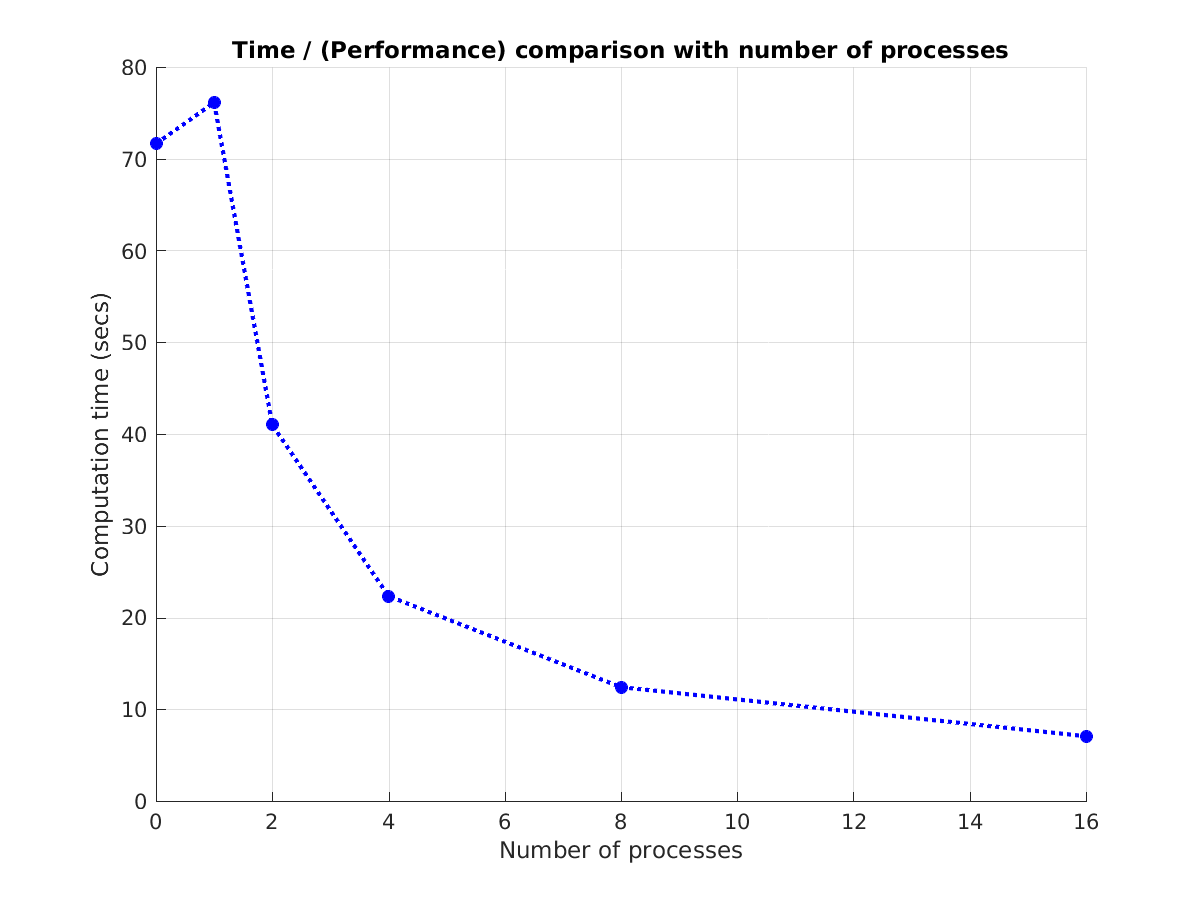
\includegraphics[width=\linewidth]{performance}
	\centering
	\label{per}
	\caption{"Performance vs No. of Processes"}
\end{figure}

\section{Conclusion}
Various OpenMP directives and clauses were used during the parallelization of the code. An insight to debug the parallelized openMP code was developed using default(none) clause. Comparing to MPI, openMP implementation is easy to use as the API hides major intricacies of breaking sequential code into parallel. 
The code in the "simulation" block inside the main, can be further parallelized to achieve better performance.
The project code/ report and generated outputs of the simulations are available at \href{https://github.com/chiragmajithia/QuakeOpenMP.git}{QuakeOpenMP} repository.

\begin{thebibliography}{1}
	
	\bibitem{notes}  Blaise Barney, Lawrence Livermore National Laboratory {\em \href{https://computing.llnl.gov/tutorials/openMP/}{webpage}}.
	
	\bibitem{impj} Tim Mattson, {\em \href{https://www.youtube.com/playlist?list=PLLX-Q6B8xqZ8n8bwjGdzBJ25X2utwnoEG}{Introduction to OpenMP - (Intel)}  }
	
	\bibitem{web}The Computational and Systems Biology (CSB) at MIT {\em \href{http://csbi.mit.edu/technology/intel_fce/doc/main_for/mergedProjects/optaps_for/ccp/optaps_par_openmp_adv_c.htm}{JOpenMP* Advanced Issues}} 
		
	
\end{thebibliography}

\end{document}
 